% !TeX root = main.tex

\section{结果分析}

\subsection{四季更替}

以 2021.03 -- 2022.03 为例, 截取 NDVI 的变化曲线如 \cref{fig:NDVI-year} 所示.
不难发现, NDVI 在春季和夏季保持较高水平, 而在秋季和冬季有所下降, 这符合大多数植被季节变化的生物学规律.
除此之外, 秋冬季节的 NDVI 波动剧烈.
这可能是由于秋冬季节气候因素多变, 大气条件不稳定, 可能导致观测受到干扰.

\begin{figure}[htbp]
  \centering
  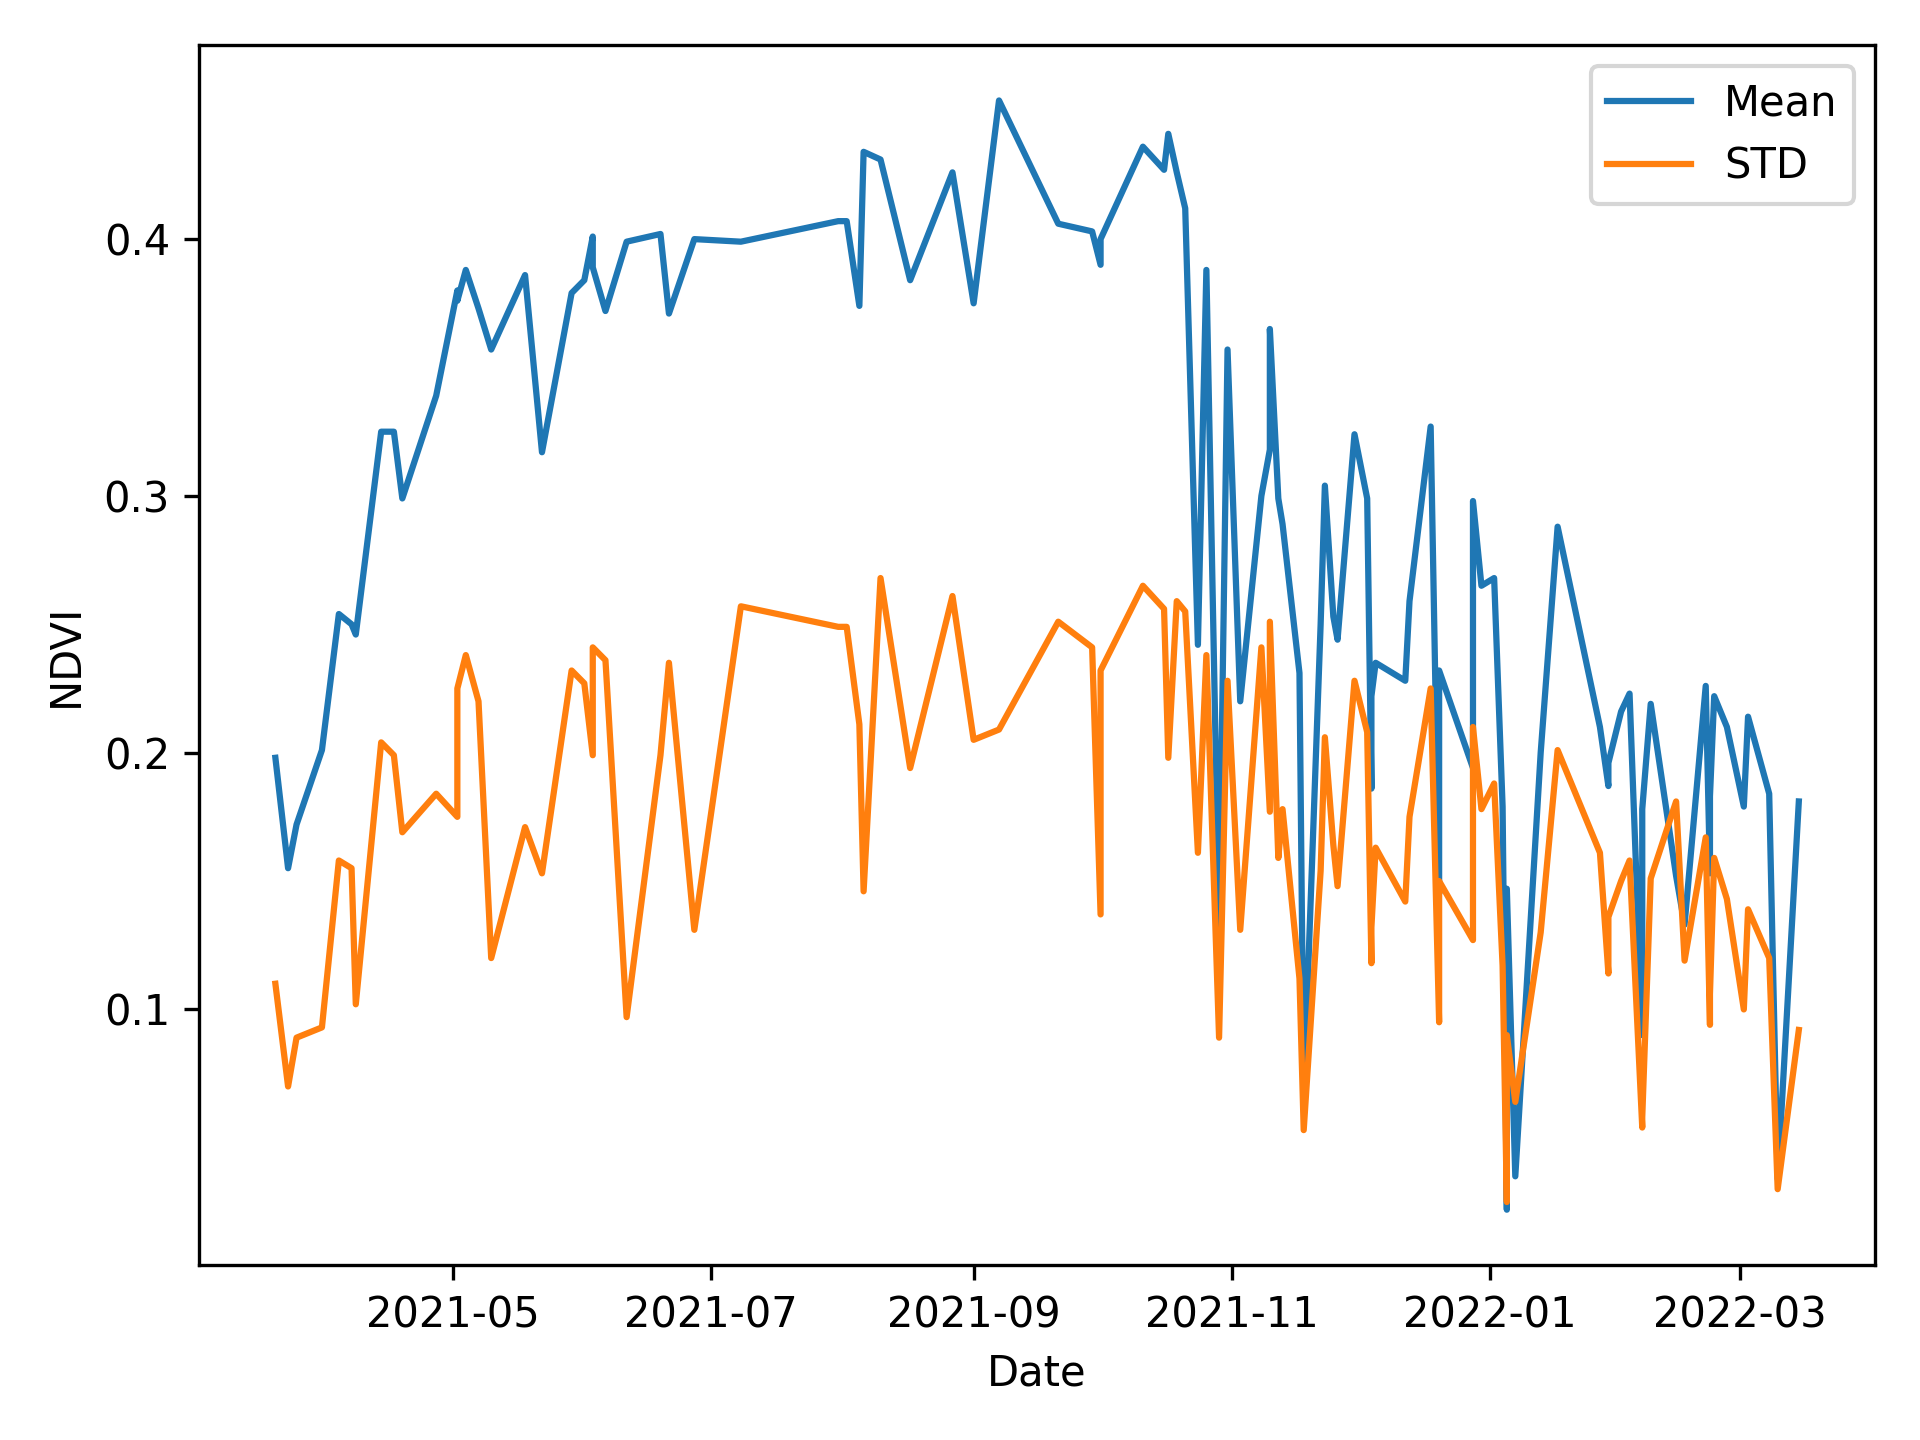
\includegraphics[width=140mm]{assets/NDVI-year.png}
  \caption{NDVI Time Series (One Year)}
  \label{fig:NDVI-year}
\end{figure}

\subsection{历史趋势}

在可用的数据范围内, 截取所有时段 NDVI 的变化曲线如 \cref{fig:NDVI} 所示.
不难看出, NDVI 年峰值在 1998 -- 2002 年出现小幅下降, 后保持稳定的缓慢增长.

值得注意的是,  NDVI 在空间分布上的标准差 (STD) 有逐渐增大的趋势, 这意味着清华校园绿化在空间分布上可能存在不均或过于集中的现象.

\begin{figure}[htbp]
  \centering
  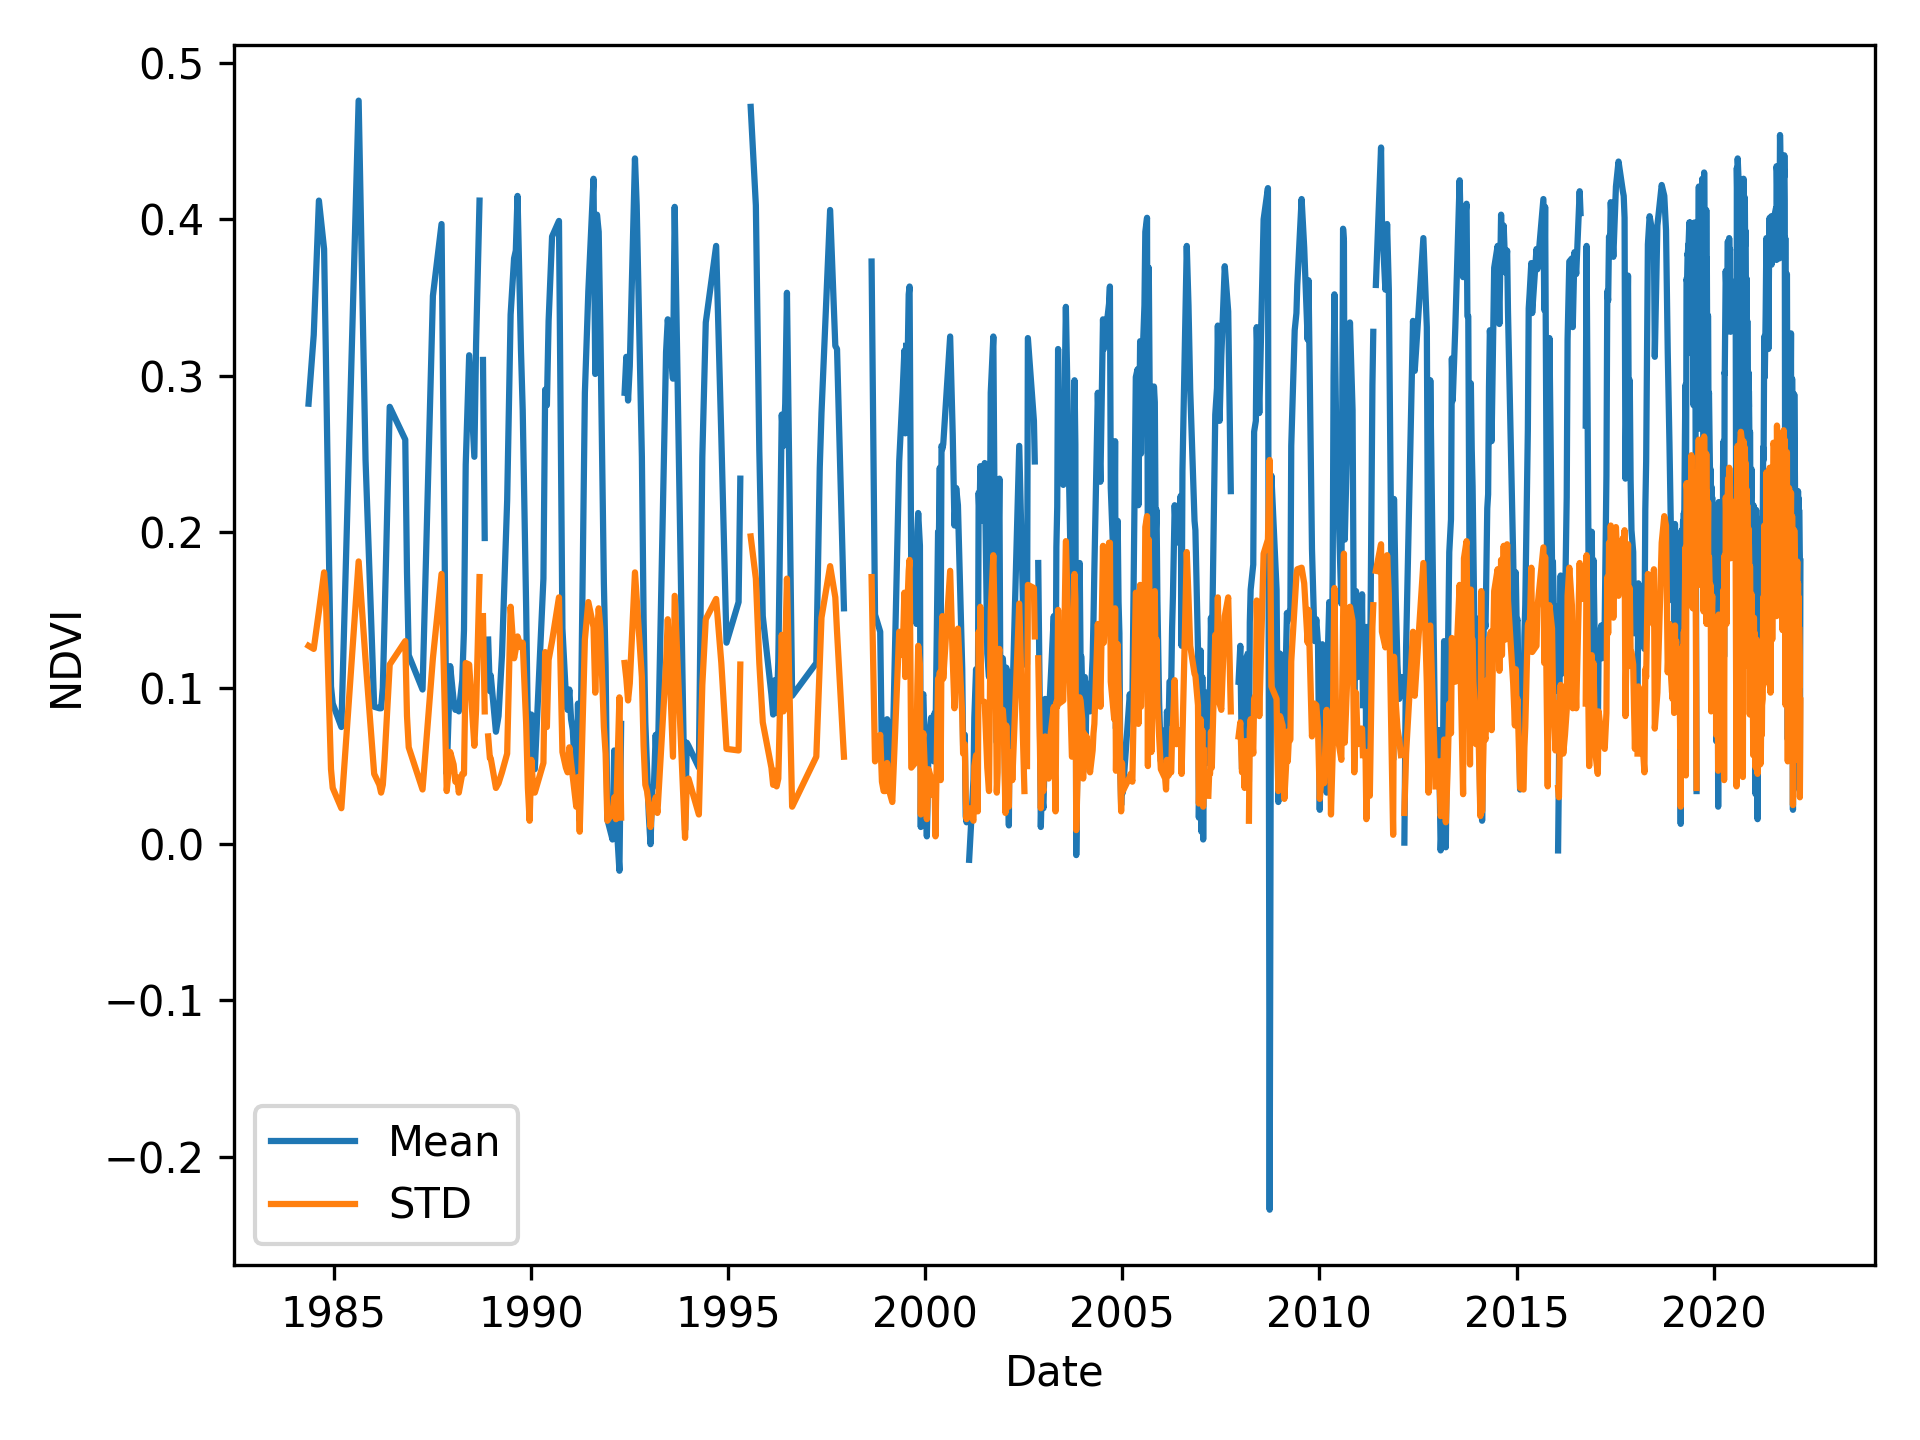
\includegraphics[width=140mm]{assets/NDVI.png}
  \caption{NDVI Time Series (All Time)}
  \label{fig:NDVI}
\end{figure}

\subsection{空间分布}

热力图能够直观反映某一时刻植被在空间上的分布情况.
以五年为周期, 选取每年 NDVI 最高的时间点作出 NDVI 的空间分布热力图如 \cref{fig:space}.
可以看出北部学生生活区的植被覆盖相比早期有所减少.

进一步地, 结合历史上的校园规划 (\cref{fig:plan}), 我们可以进行更加细致的分析.
可以看出校园中绿地区域, 如树林、操场天然草坪等, 与热力图中 NDVI 较高的区域基本吻合.

\begin{figure}[htbp]
  \centering
  \subcaptionbox{Map}{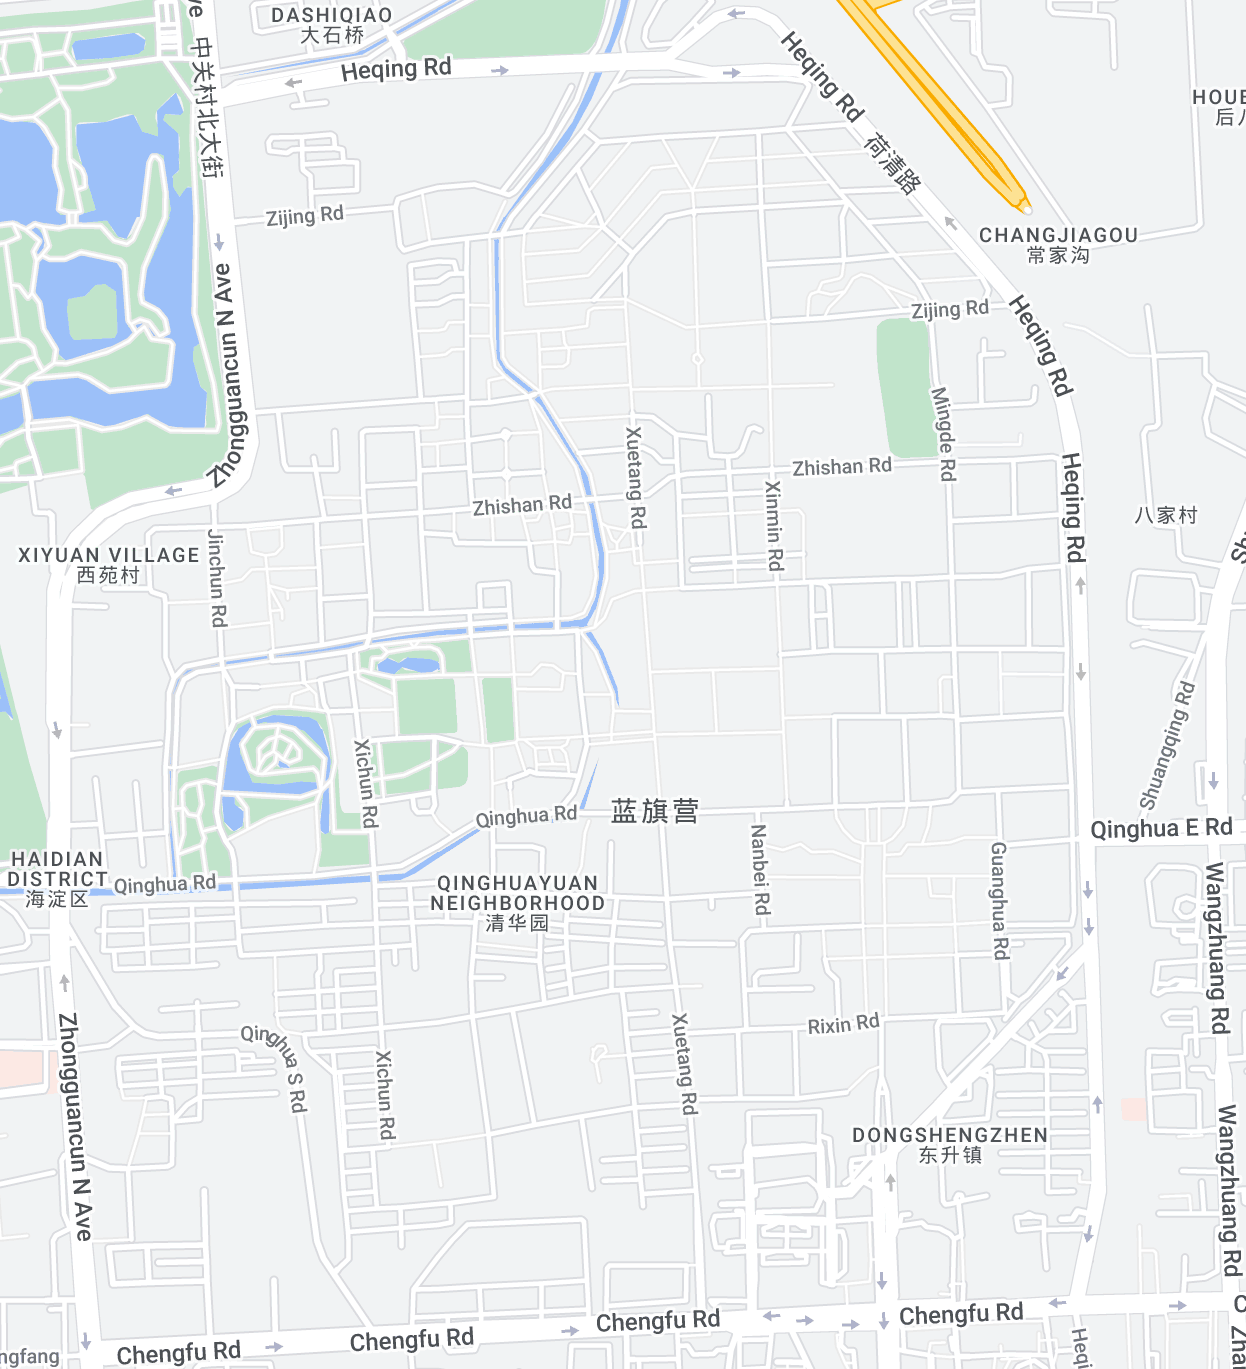
\includegraphics[height=0.25\linewidth]{assets/plain.png}}
  \quad
  \subcaptionbox{1985-08-19}{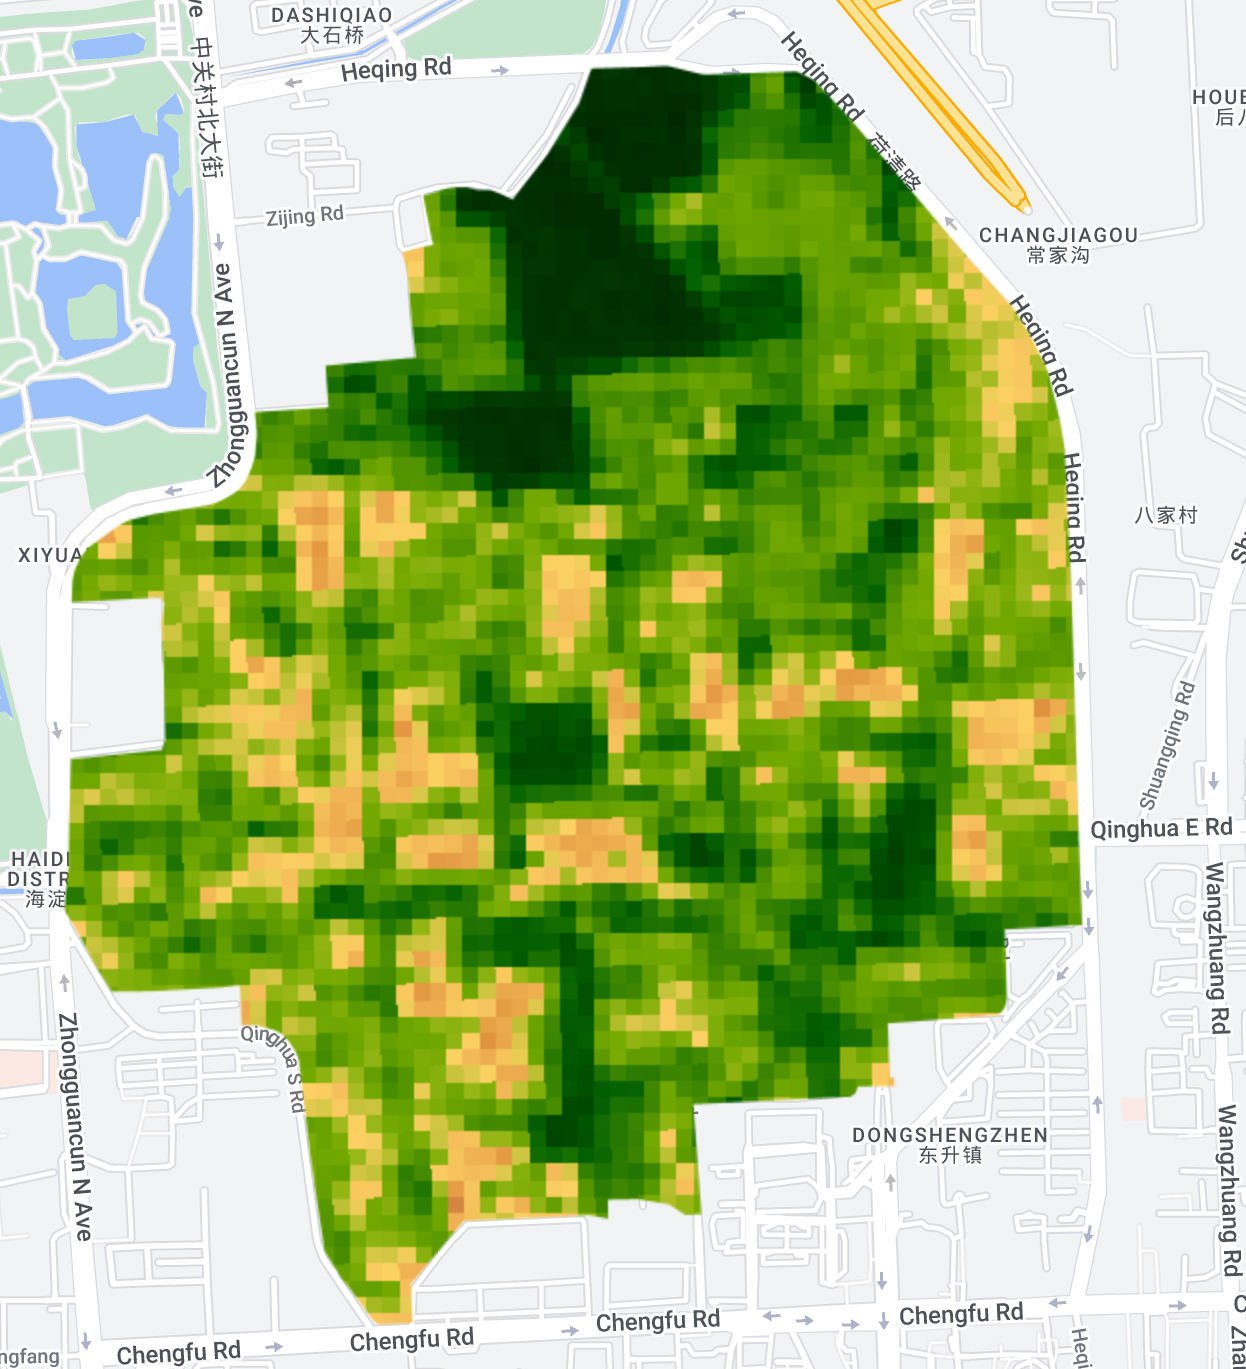
\includegraphics[height=0.25\linewidth]{assets/1985-08-19.png}}
  \quad
  \subcaptionbox{1990-09-18}{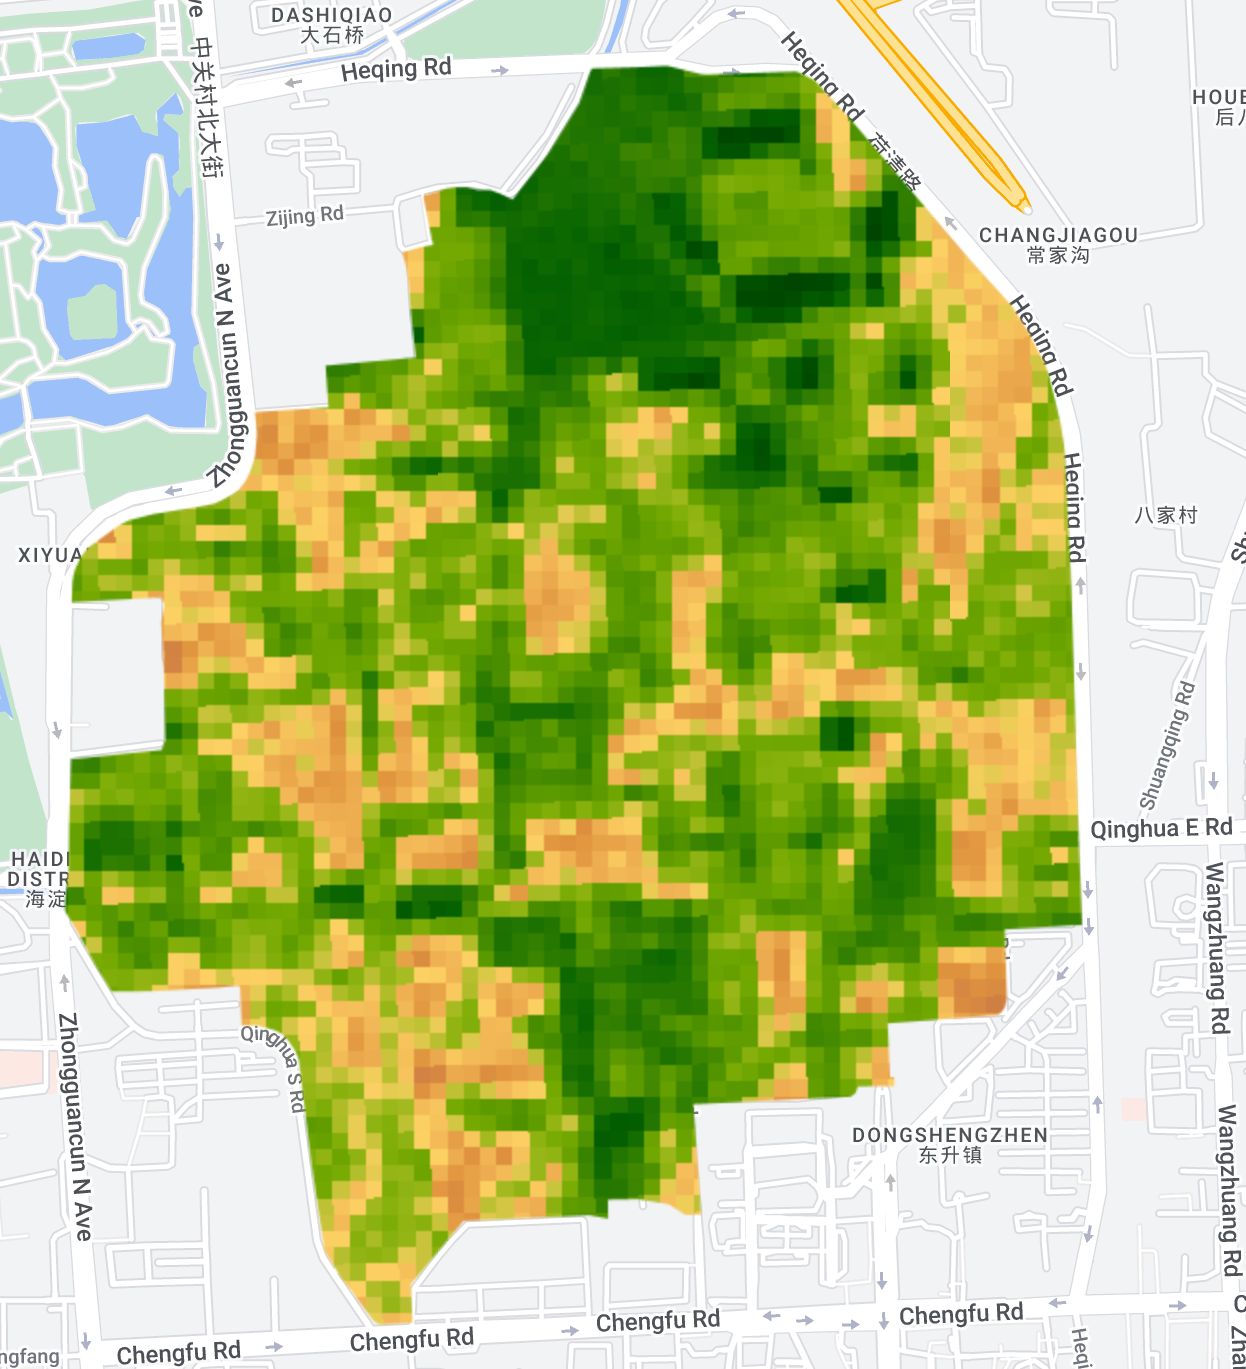
\includegraphics[height=0.25\linewidth]{assets/1990-09-18.png}}
  \quad
  \subcaptionbox{1995-07-30}{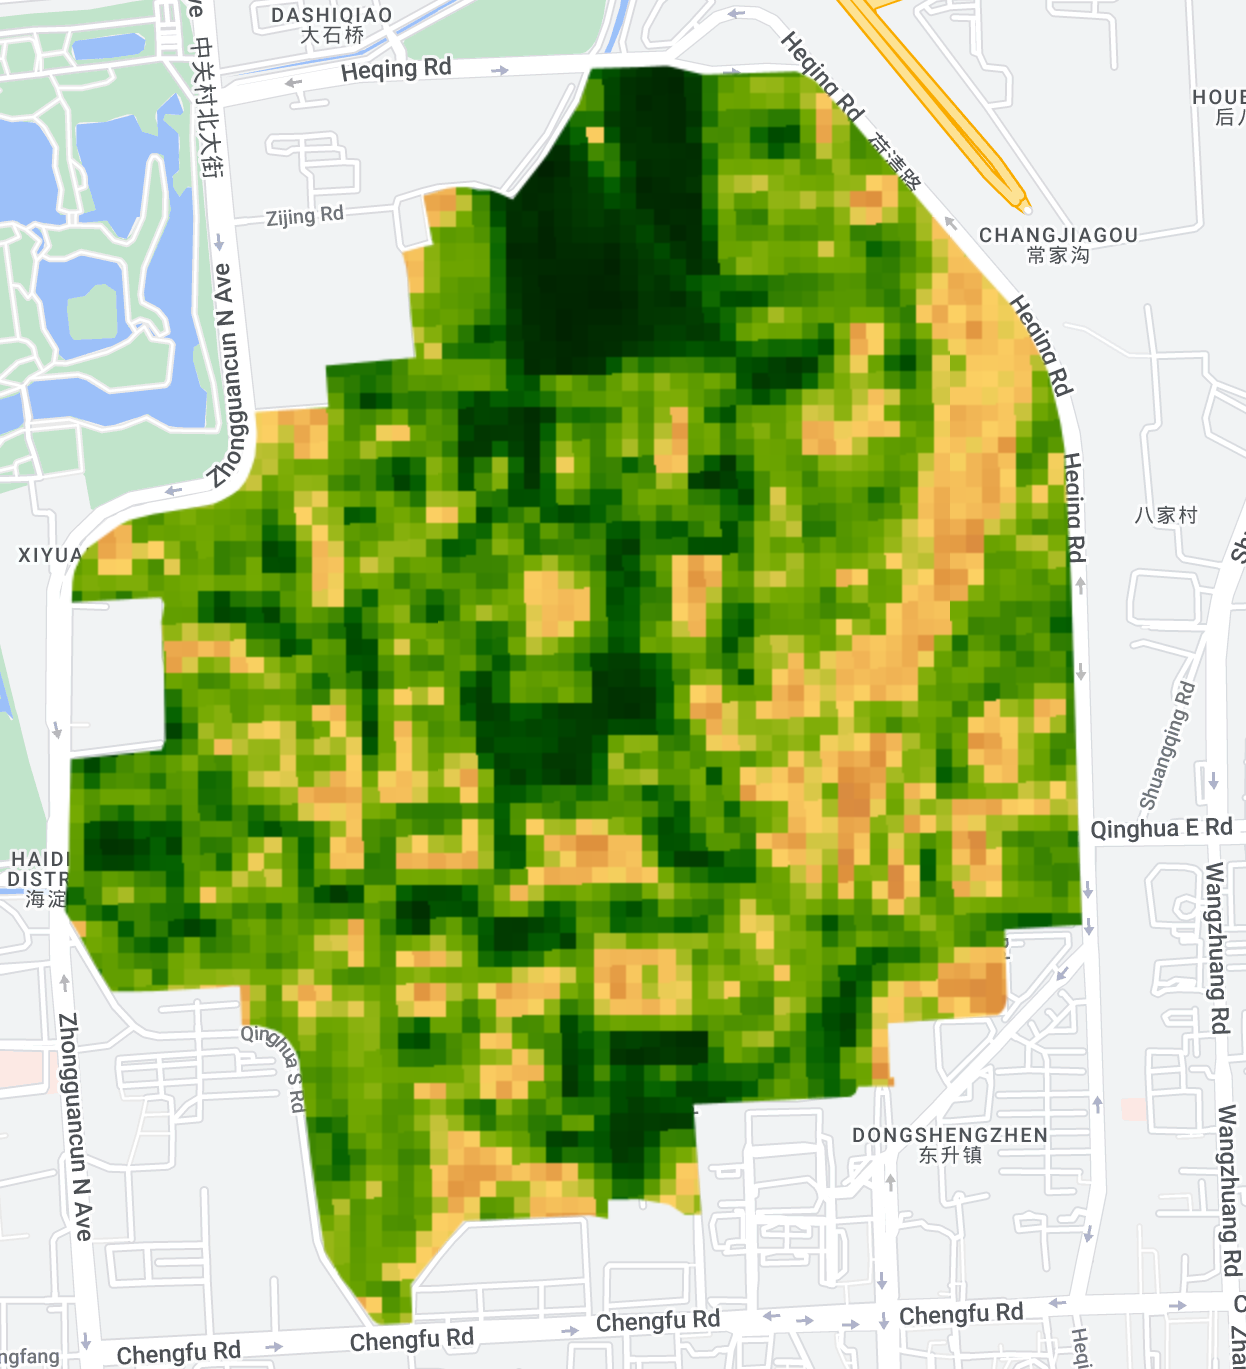
\includegraphics[height=0.25\linewidth]{assets/1995-07-30.png}}
  \quad
  \subcaptionbox{2000-08-20}{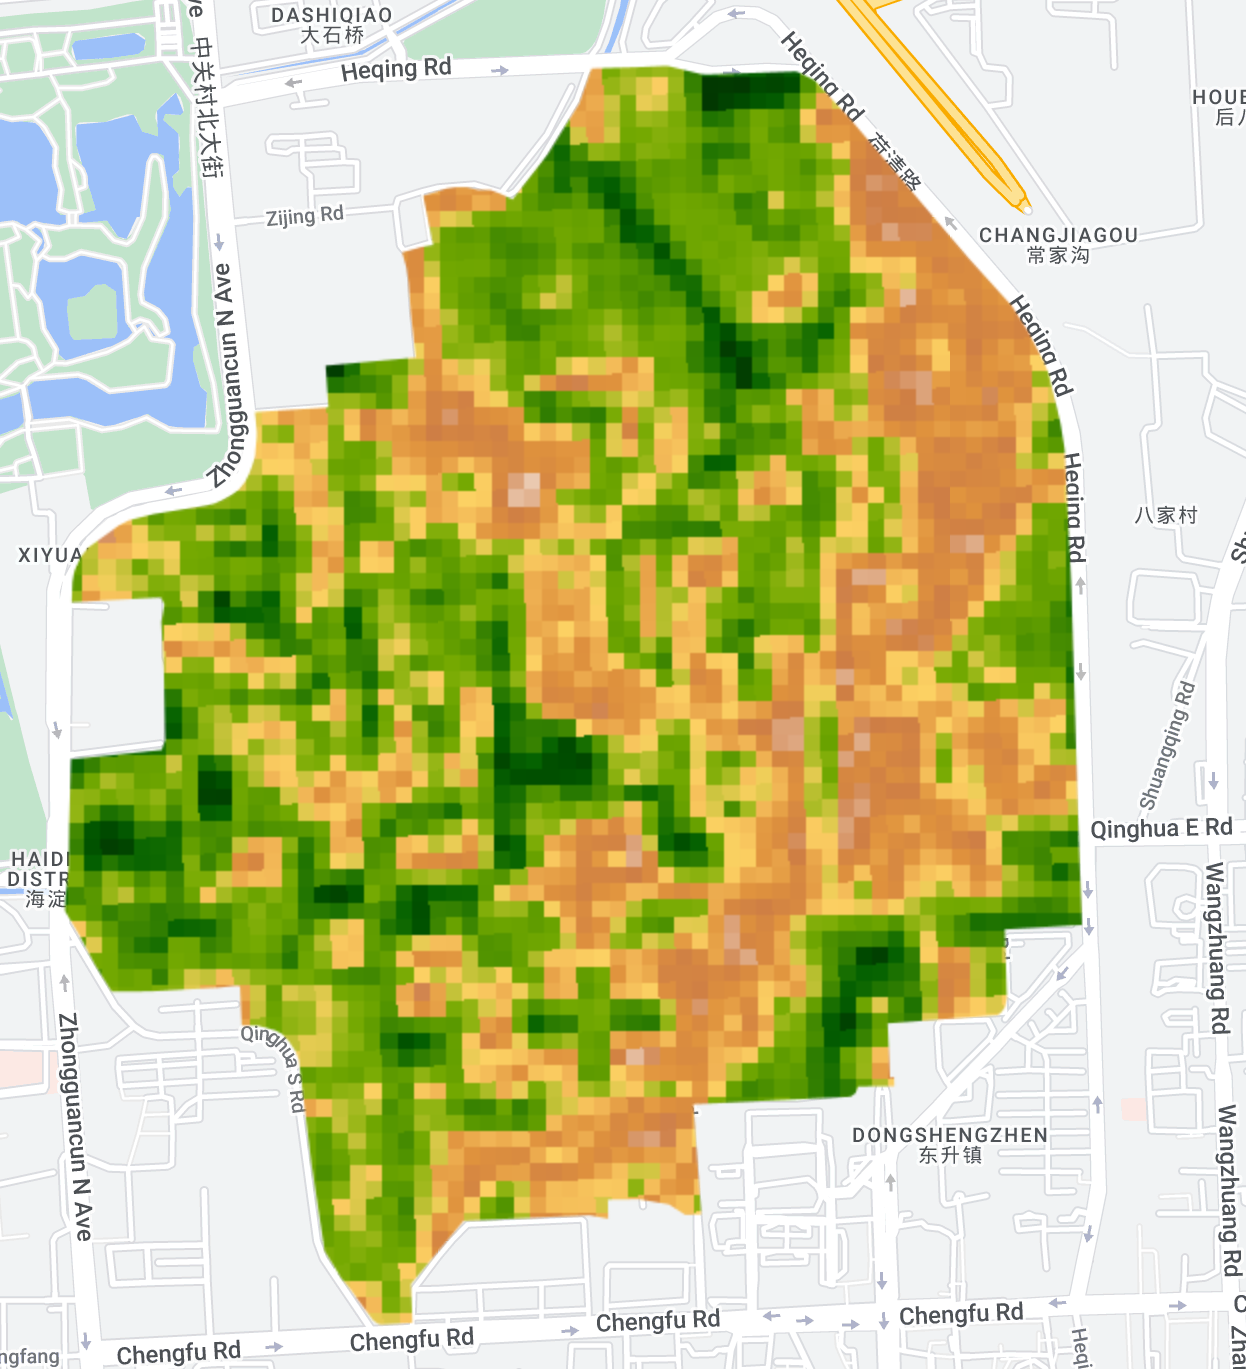
\includegraphics[height=0.25\linewidth]{assets/2000-08-20.png}}
  \quad
  \subcaptionbox{2005-08-18}{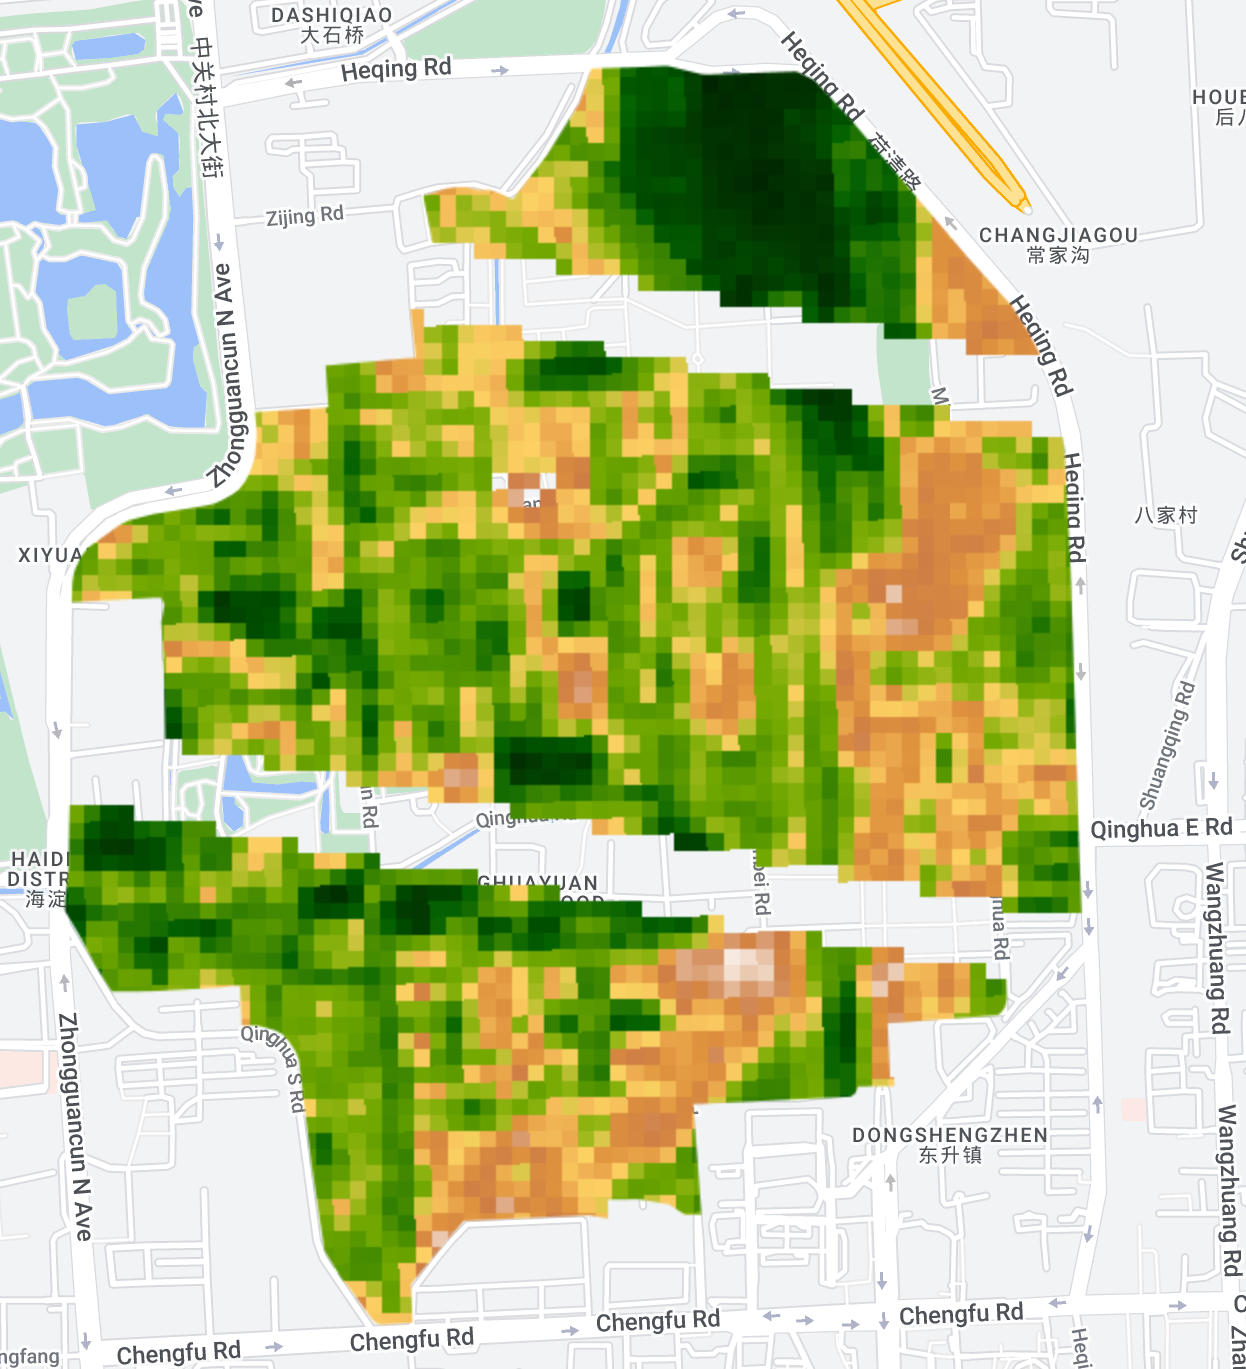
\includegraphics[height=0.25\linewidth]{assets/2005-08-18.png}}
  \quad
  \subcaptionbox{2010-08-08}{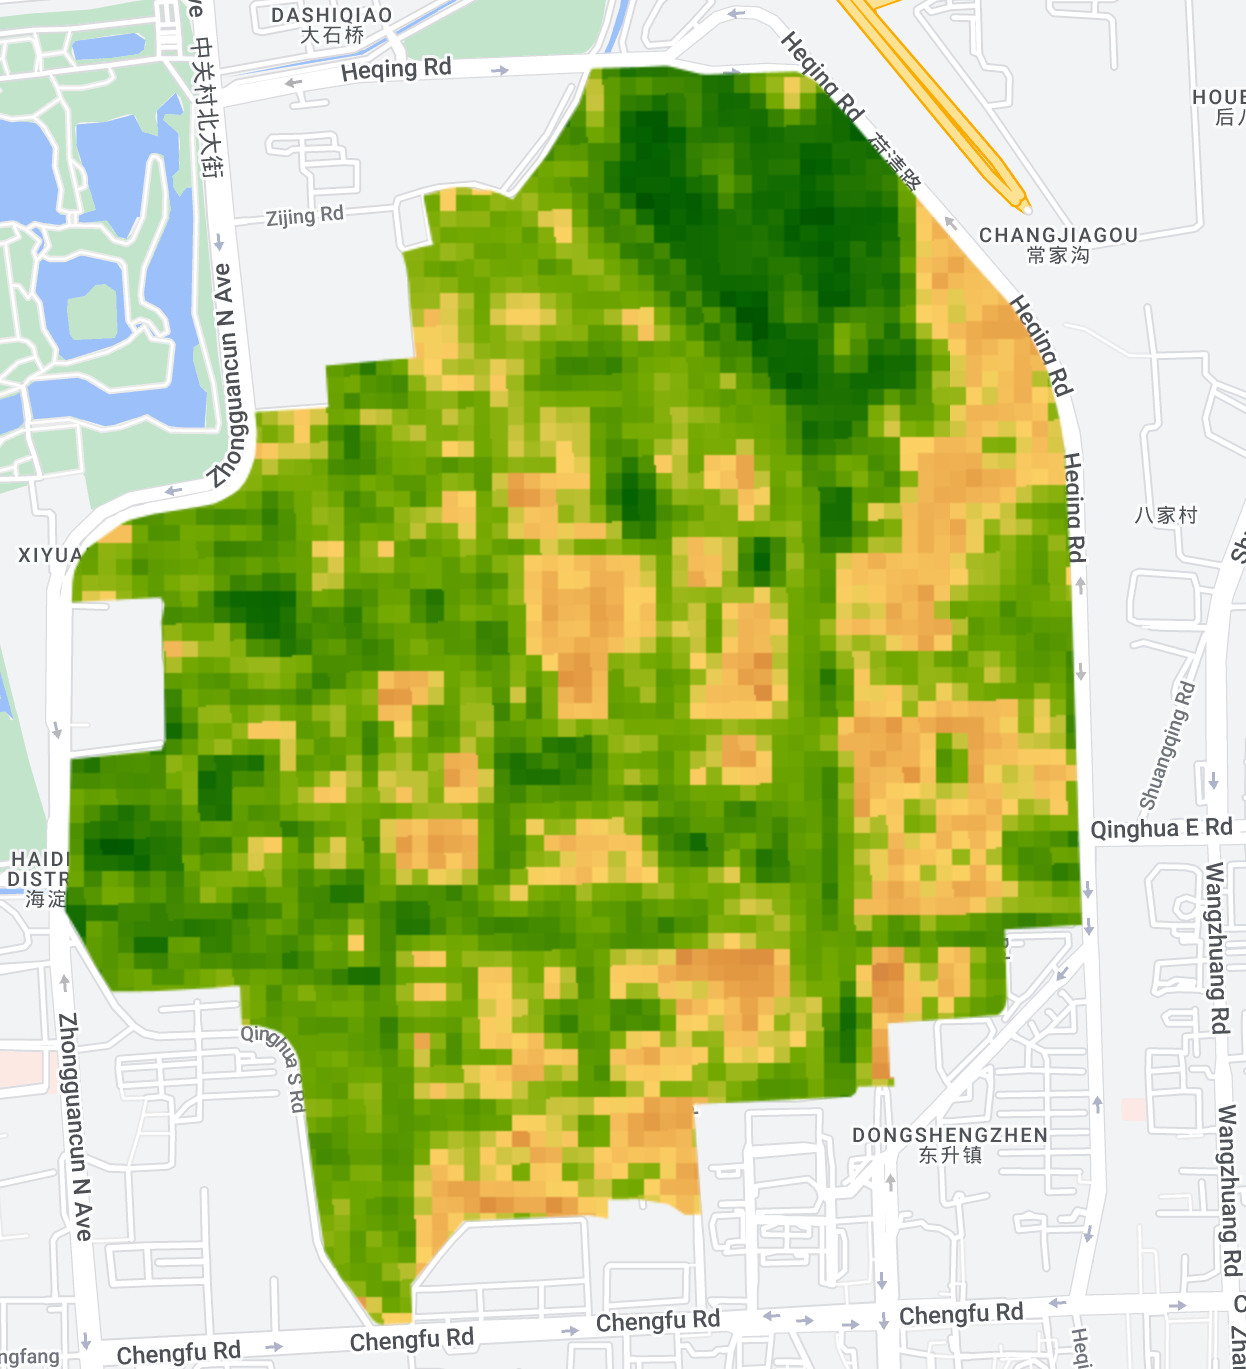
\includegraphics[height=0.25\linewidth]{assets/2010-08-08.png}}
  \quad
  \subcaptionbox{2015-09-07}{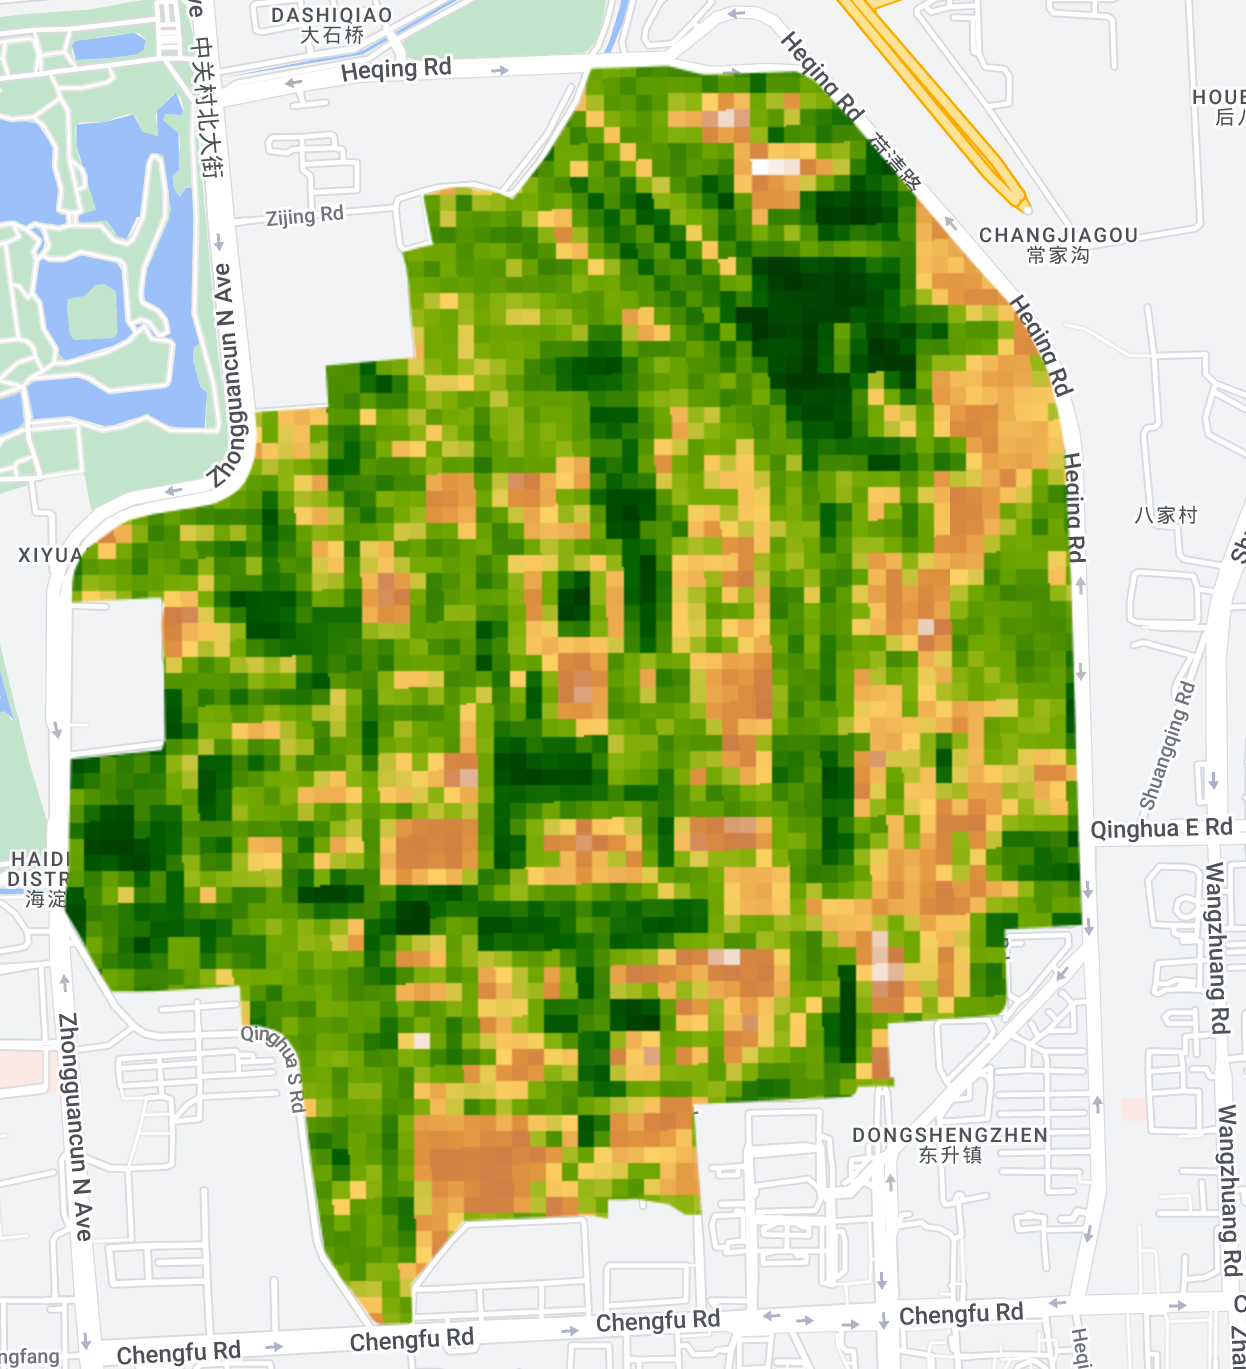
\includegraphics[height=0.25\linewidth]{assets/2015-09-07.png}}
  \quad
  \subcaptionbox{2020-08-11}{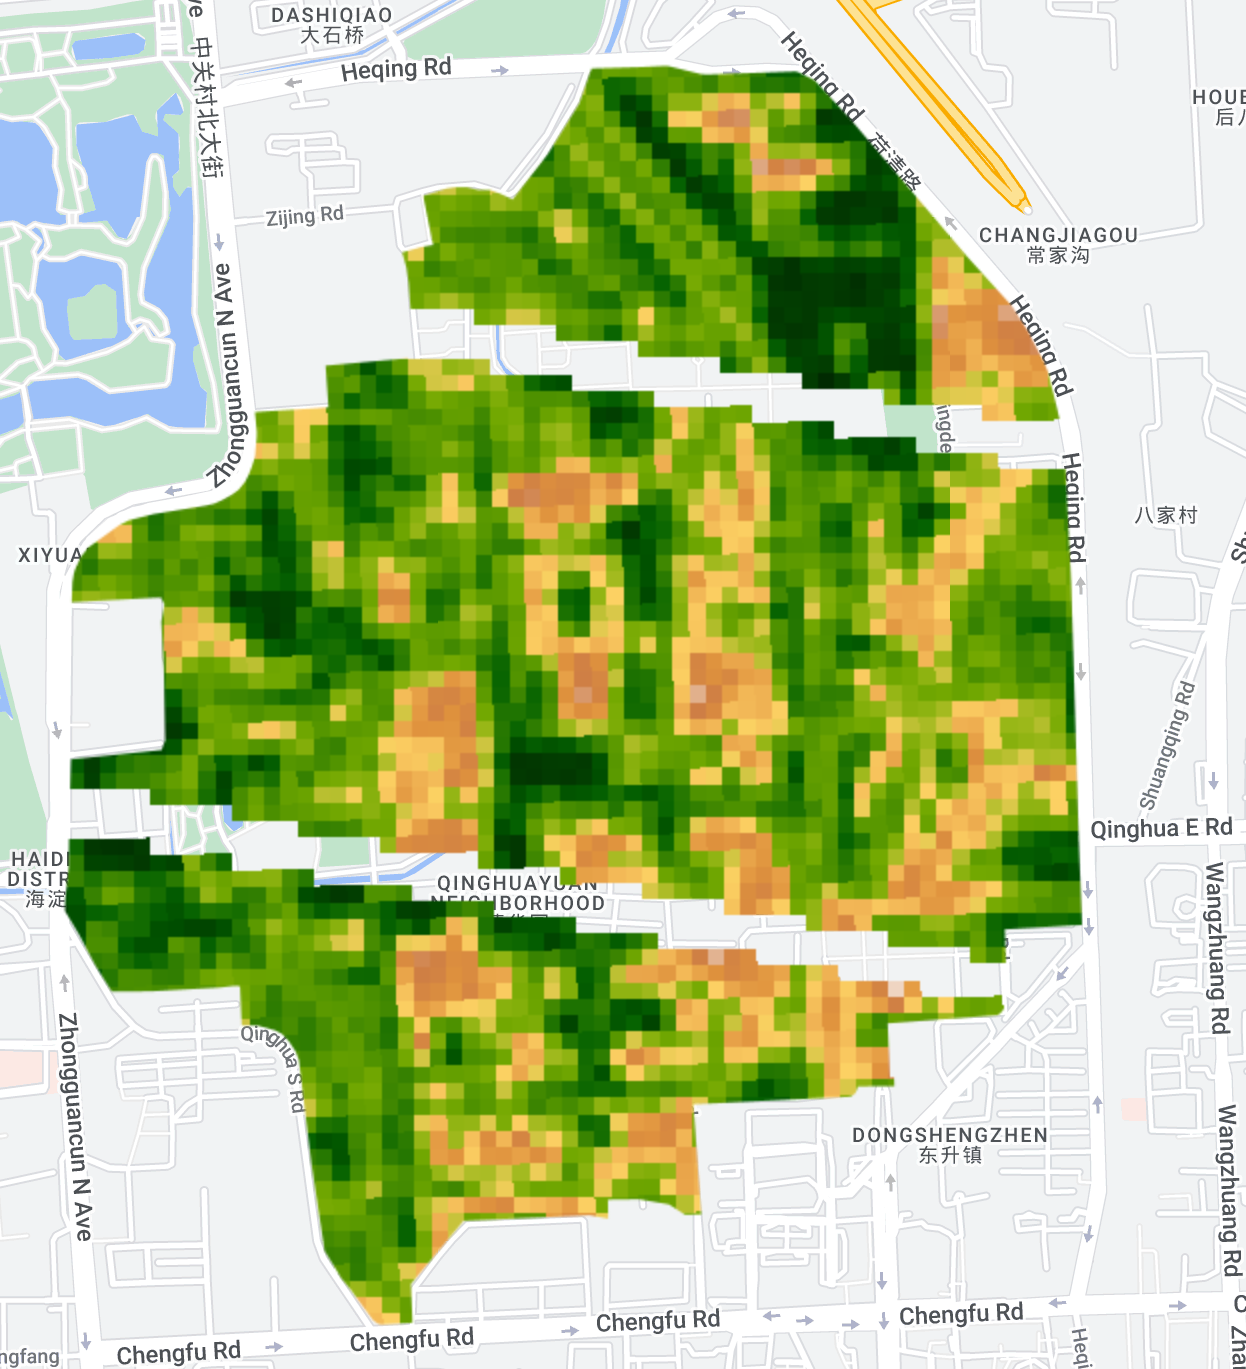
\includegraphics[height=0.25\linewidth]{assets/2020-08-11.png}}
  \quad
  \subcaptionbox{2022-01-17}{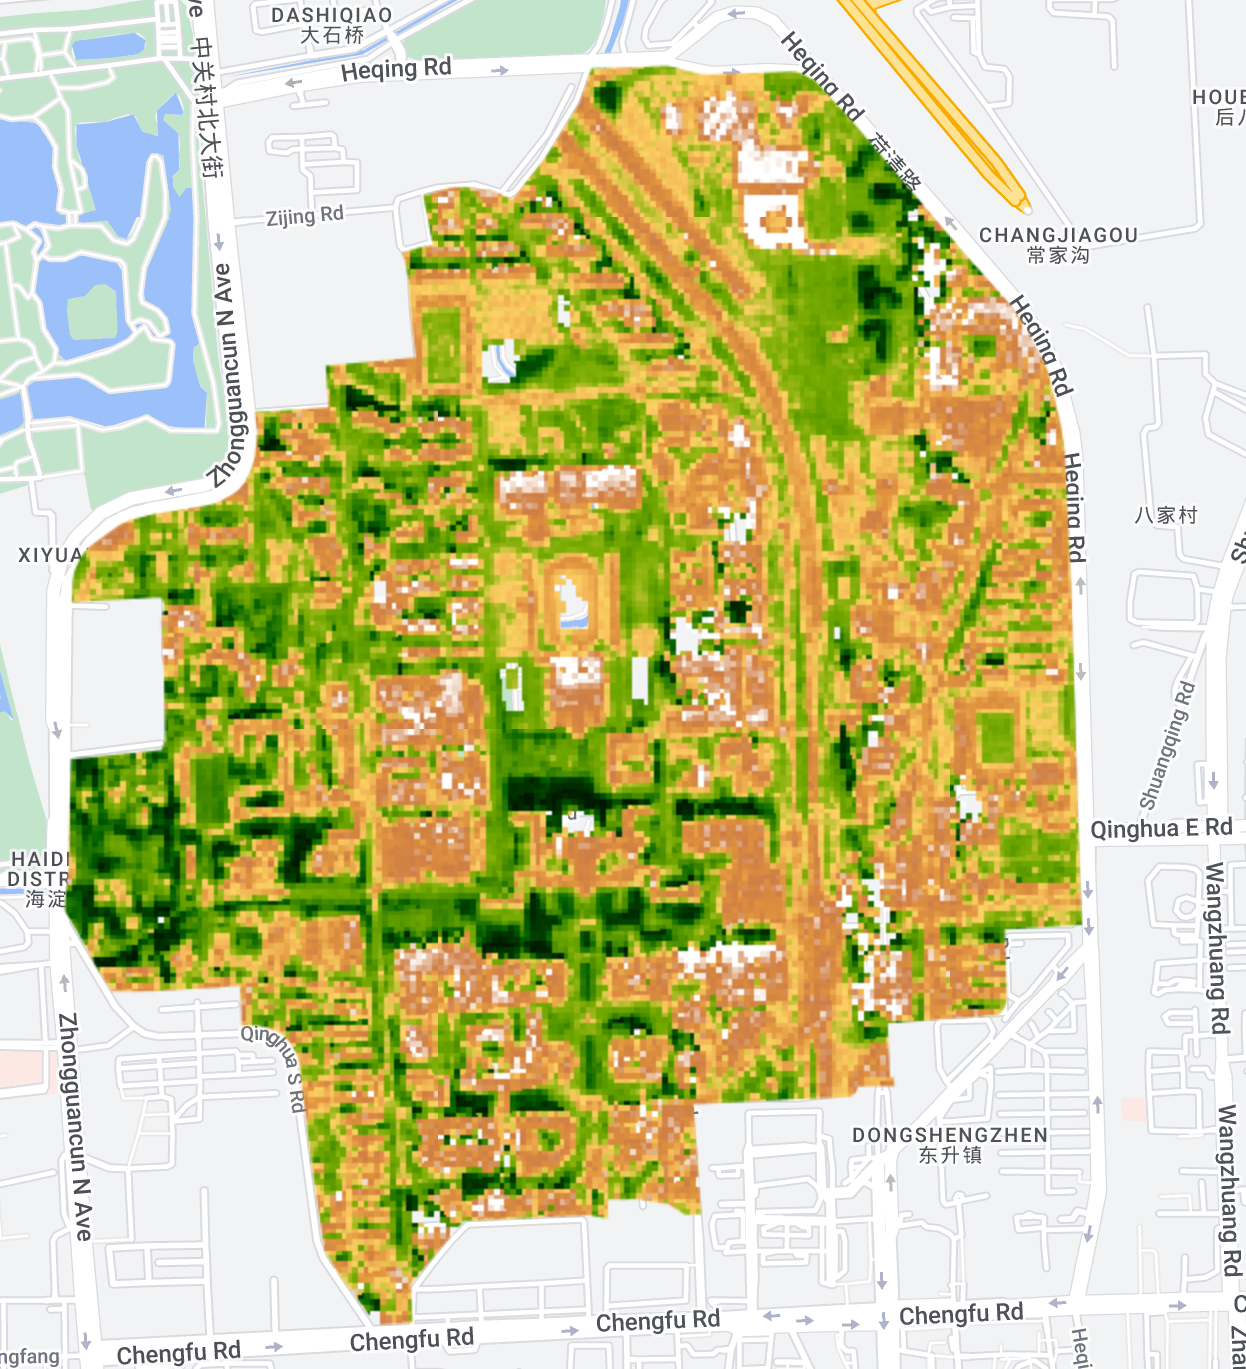
\includegraphics[height=0.25\linewidth]{assets/2022-01-17.png}}
  \quad
  \caption{NDVI 热力图}
  \label{fig:space}
\end{figure}

\begin{figure}[htbp]
  \centering
  \subcaptionbox{1988 年清华校园规划}{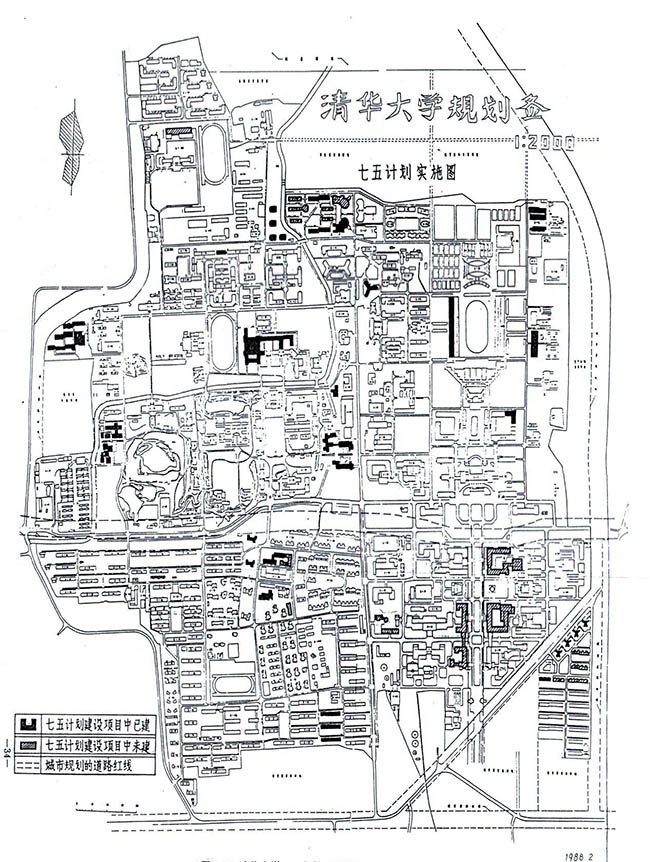
\includegraphics[height=0.3\linewidth]{assets/plan-1988.jpg}}
  \quad
  \subcaptionbox{1994 年清华校园规划}{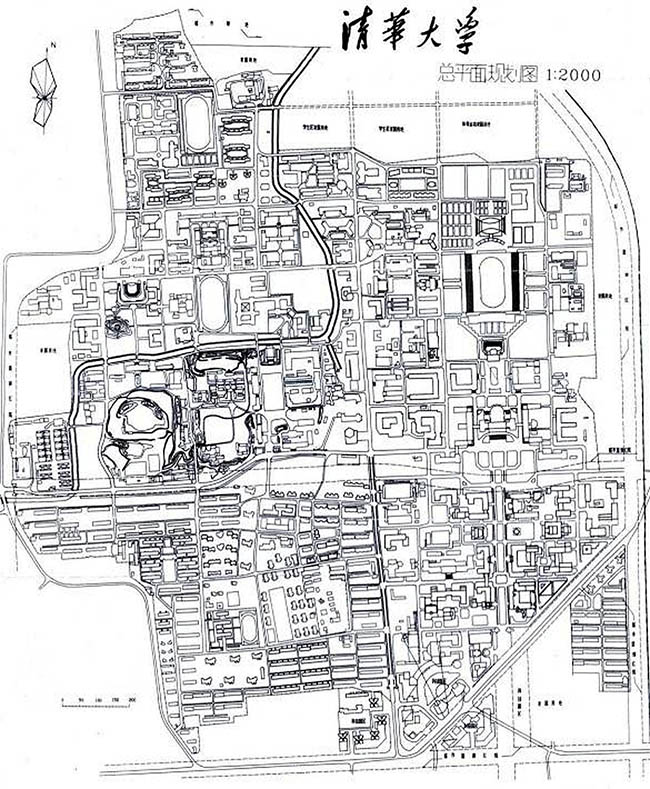
\includegraphics[height=0.3\linewidth]{assets/plan-1994.jpg}}
  \quad
  \subcaptionbox{2021 年校园地图}{\includegraphics[height=0.3\linewidth]{assets/plan-2021.jpeg}}
  \quad
  \caption{校园规划}
  \label{fig:plan}
\end{figure}
